\begin{table}[b]
\begin{center}
\begin{tabular}{@{}cc@{}}
\toprule
\textbf{Pretraining} & \textbf{Average EAI Results}\\
\midrule
English-only  & \textbf{41.72}\\
Multilingual  & 38.55\\
\bottomrule
\end{tabular}
\end{center}
\caption{\textbf{Multilingual pretraining very significantly diminishes English zero-shot generalization.} Both models trained on OSCAR for 112B tokens.}
\label{tab:mutlilingual}
\end{table}




The majority of 100B+ language models have been trained in English, with notable exceptions in Chinese~\citep{zeng2021pangu, wu2021yuan} and Korean~\cite{Kim2021WhatCC} models. Smaller massively multilingual models have seen wider adoption \cite{mT5}, but these models are not suitable for zero-shot. Recent results on large GPT-like multilingual models show that English-only performance is usually disappointing \cite{XGLM}. 

\paragraph{Training data.}
We train a multilingual model to evaluate the effectiveness and potential impacts of this practice. 
We use the OSCAR dataset~\citep{ortiz2019oscar}, but here we include multiple languages, not only English as in the earlier experiments. 
The languages we include are Arabic, Basque, Bengali, Chinese, Catalan, English, French, Hindi, Indonesian, Portuguese, Spanish, Urdu, and Vietnamese.
We sample each language with a different probability that downsamples the most frequent languages 
and upsamples the least frequent ones, so that all languages 
are represented. We estimate the sampling probabilities similar to~\citet{Xue2021mT5AM}.




\paragraph{English-only evaluation.}
We first evaluate our multilingual model on the same set of English benchmarks we have used previously, in Table~\ref{tab:mutlilingual}. Multilinguality significantly lowers accuracy on the English benchmark, which is in line with the results from~\citet{XGLM}. 

\paragraph{Multilingual evaluation.}
Zero-shot multilingual evaluation is more challenging to setup because it requires writing new prompts for each new language. Therefore, instead of manually writing prompts for each language, we follow the strategy proposed by~\citet{XGLM}, using English prompts for non-English examples--this can be viewed as cross-lingual zero-shot generalization. They validated this strategy by demonstrating its ability to achieve zero-shot performance on par with (and sometimes even better than) human-written language-specific prompts. This strategy also demonstrates cross-lingual abilities.

\definecolor{shadecolor}{rgb}{0.93,0.93,0.93}


We evaluate on XNLI~\citep{conneau2018xnli}, a multilingual NLI dataset  that covers 8 of the languages we use for training. 
%The task uses the following English cloze-style prompt template across all languages: \colorbox{shadecolor}{\texttt{[premise]}, right? \texttt{[MASK]}, \texttt{[hypothesis]}} The prompt fields, \texttt{[premise]} and \texttt{[hypothesis]}, are filled with the premise/hypothesis pairs in the target language. 
%For zero-shot evaluation, the \texttt{[MASK]} token is replaced with ``Yes'' (for entailment), ``No'' (for contradiction) and ``Also'' (for neutral). The completion with the highest likelihood according to the model is taken as its prediction.
Our evaluation is different from the zero-shot evaluation of the XTREME benchmark~\cite{Hu2020XTREMEAM}. XTREME first finetunes the model on the English training data of each downstream task, then evaluates it on the non-English dataset, attempting cross-lingual generalization. 
Our evaluation avoids any finetuning, and instead relies entirely on zero-shot generalization.
 

\paragraph{Results.}
Table~\ref{tab:mutlilingual_xnli} shows the XNLI results of our multilingual model and how it compares to XGLM~\cite{XGLM}.
We were able to reproduce the results of XGLM-7.5B which validates our evaluation setup. Furthermore, the table shows that the performance of our 1.3B 
is in line with the XNLI 1.7B model, validating that our multilingual setup achieves competitive results. It is worth noting that our 1.3B model is trained on only 112B tokens from 13 languages while 
XGLM is trained on 500B tokens from 30 languages. As far as we are aware, this is the first independent replication of the main results of~\citet{XGLM}.

\paragraph{Language-specific scaling laws.} To explore how scale influences multilinguality, we train a wider range of models (i.e. 0.3-6B parameters) on a larger corpus of more than 300B tokens of text drawn from a variety of languages \cite{roots}. In Figure \ref{fig:multilingualscaling}, we show scaling laws for Arabic, Catalan, Code, English, Spanish, Basque, French, Indonesian, Assamese, Bengali, Gujarati, Hindi, Kannada, Malayalam, Marathi, Nepali, Odia, Punjabi, Tamil, Telugu, Urdu, aggregated Niger-Congo languages, Portuguese, Vietnamese, Simplified and Traditional Chinese. 

Smaller models struggle more with under-represented languages such as those in the Indic and Niger-Congo family. For example, the loss of the sub-1 billion models goes up at the end of training for Malayalam, Odia, and Telugu. As data is not repeated, it is unlikely that this effect is due to overfitting; we interpret this as insufficient capacity in the model to handle many language representations, with data in the dominant language sets causing catastrophic forgetting of less represented languages. In contrast, the largest model sees its loss decrease smoothly for every language: larger models handle multilinguality more easily. Overall, scaling laws coefficients are consistent across well-represented languages, only differing in offsets.

\begin{figure*}[t]
    \centering
    \centerline{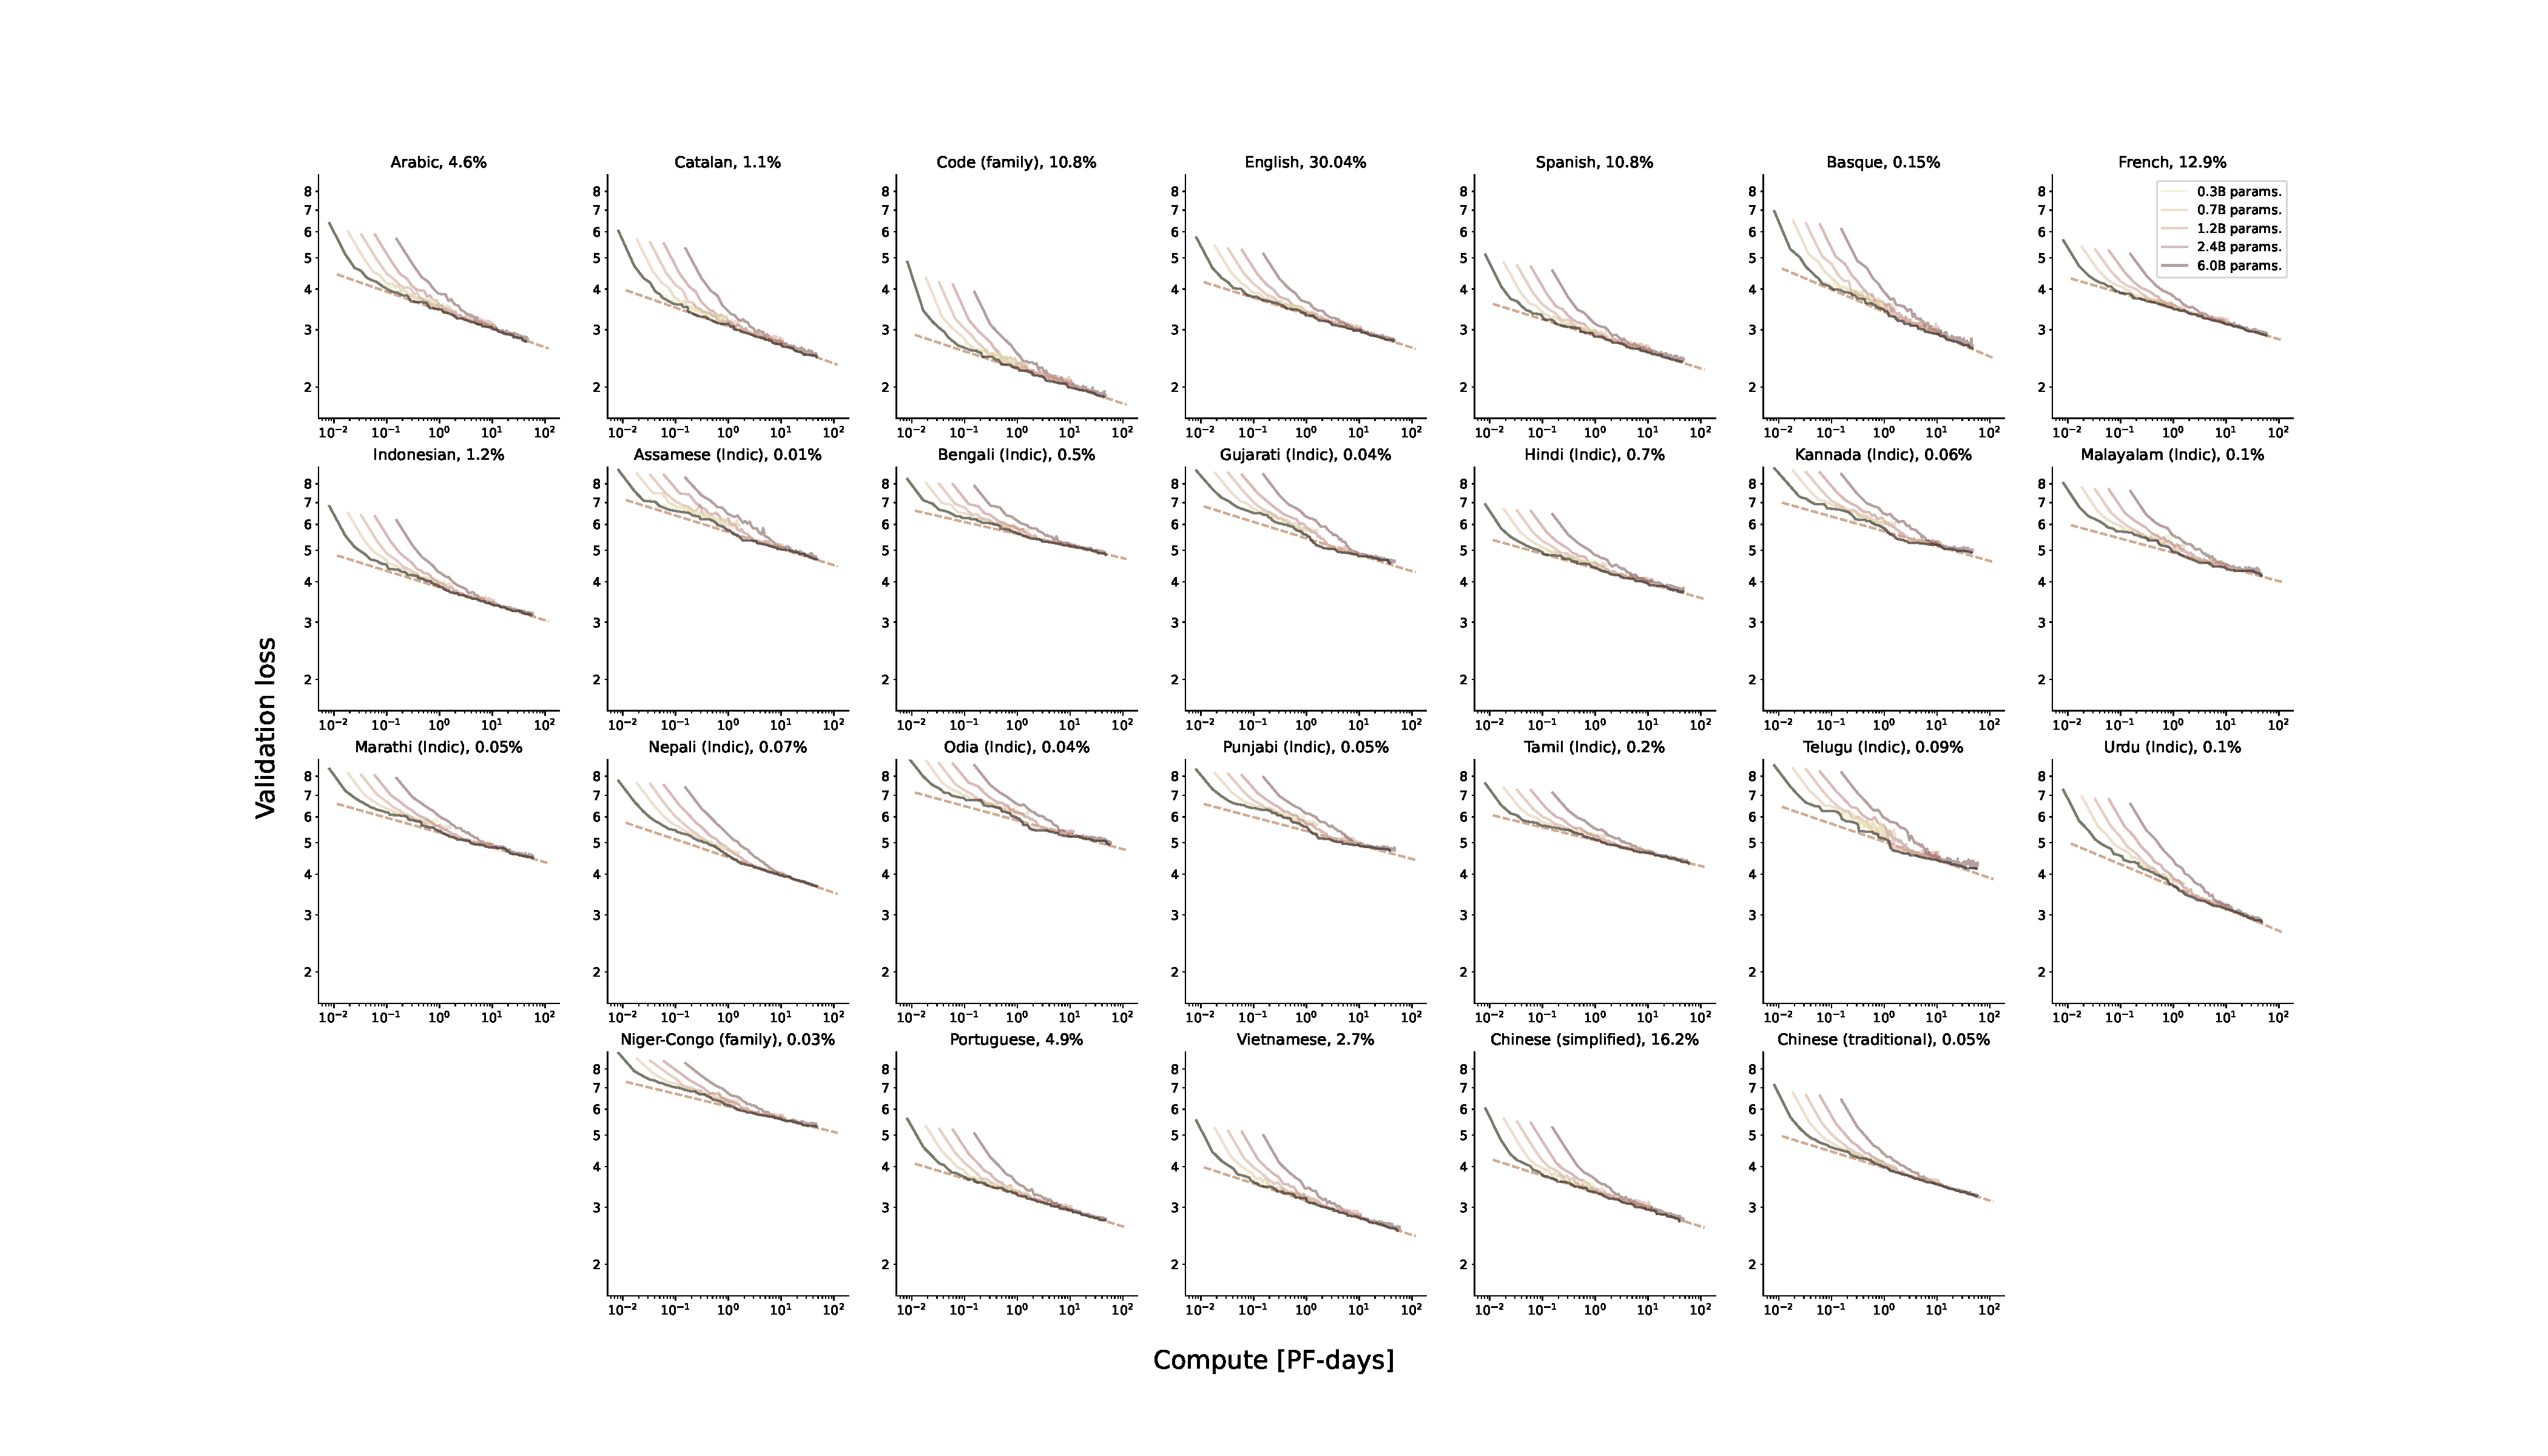
\includegraphics[width=1.1\textwidth]{figures/multilingual_scaling.pdf}}
    \caption{\textbf{Scaling laws across languages for the smaller BLOOM models}. Black line is Pareto frontier of optimality (best loss at a given compute), dashed line is best fit. Fit coefficients are detailed in Appendix \ref{sec:multilingualscalinglaws}. All sufficiently represented languages exhibit similar scaling behaviour, with mostly differences in loss offsets.}
    \label{fig:multilingualscaling}
\end{figure*}